\chapter{Results}
\label{ch:results}

Presented in this chapter are the results obtained by applying the previously described methods. Due to uncertain normalization
factors, all values are given with respect to the maximum charm component in terms of flux $\dot{\phi}_\nu$ or fluence $\phi_\nu$
for physical quantities. As per its definition,
\begin{equation}
	\dot{\phi}_\nu \kern+0.25pt = \frac{d \kern+0.75pt \dot{N}_{\kern-0.5pt \nu} / \kern-1.0pt dE_\nu \kern+0.25pt}{4\pi d^2} \:,
	\label{eqn:flux}
\end{equation}
the flux counts neutrinos per energy, time and area. Equation \eqref{eqn:flux} derives from evenly spreading all spectral
intensity over a spherical surface with radius equal to the distance $d \kern+0.5pt$ from a single source. Integrating over
time yields the fluence
\begin{equation}
	\phi_\nu \kern+0.25pt = \frac{dN_{\kern-0.5pt \nu} / \kern-1.0pt dE_\nu \kern+0.25pt}{4\pi d^2} \:,
	\label{eqn:fluence}
\end{equation}
which measures neutrino numbers per energy and area instead. Because $d \kern+0.5pt$ is a constant, forming ratios of
$\dot{\phi}_\nu$ or $\phi_\nu$ eliminates it. Accordingly, the following results are distance independent.

\begin{figure}[H]
	\centering
	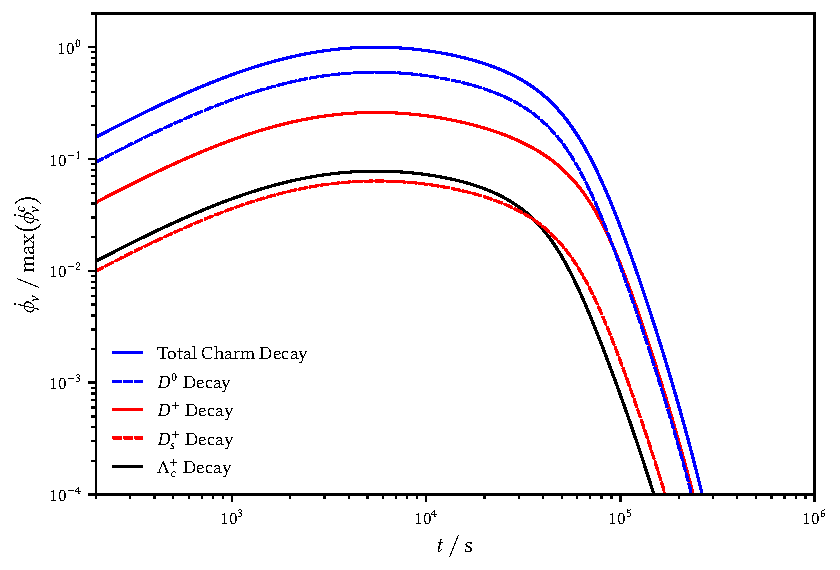
\includegraphics{../plots/build/magnetar_charm_decay_comparison_with.pdf}
	\caption[Magnetar $\nu \kern+0.5pt$ flux from $c$ decay including optical depth.]
			{Comparison of individual charmed hadron contributions to the total charm neutrino flux at
			 $E_\nu = \kern-0.5pt \qty{e9}{\giga\electronvolt}$ from a young magnetar, including the optical
			 depth defined by \eqref{eqn:optical} as a modification. Decays of $\smash{D^0}$ produce most of
			 the charmed neutrinos until later times when $\smash{D^+} \kern-0.5pt$ becomes significant, with
			 $\smash{D^+_s}$ and $\smash{\Lambda^{\kern-0.5pt +}_{\kern+0.5pt c}}$ being similar, both
			 contributing around \qty{10}{\percent} to the combined flux. This is in line with the
			 cross sections from \ref{sub:charm} as well as the branching fractions that
			 Table \ref{tab:charm-hadrons} lists.}
	\label{fig:magnetar-charm-comparison-with}
\end{figure}


\begin{figure}[H]
	\centering
	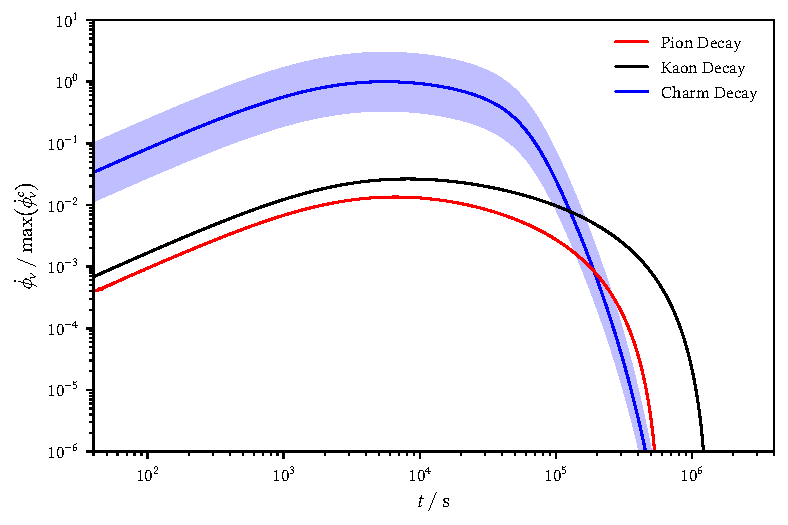
\includegraphics{../plots/build/magnetar_neutrino_spectrum_with.pdf}
	\caption[]{}
	\label{fig:magnetar-flux-with}
\end{figure}

\vfill
\begin{figure}[H]
	\centering
	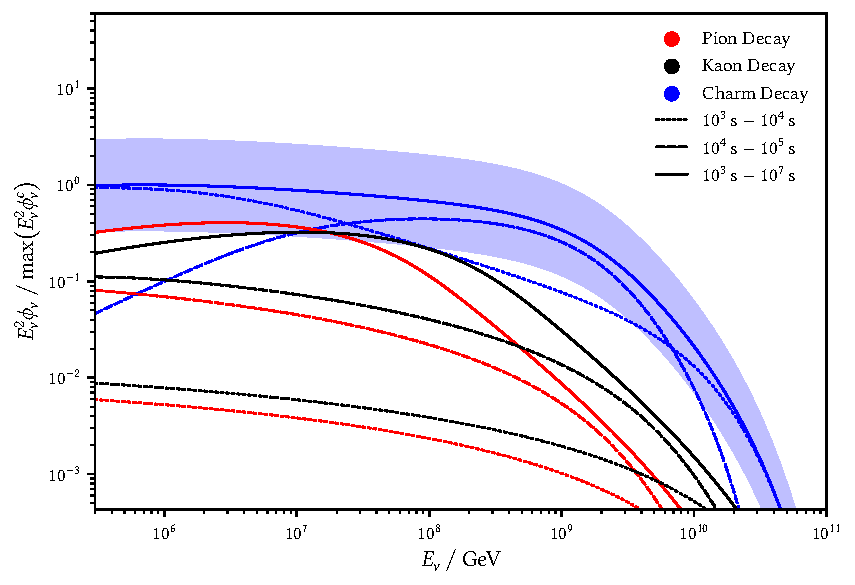
\includegraphics{../plots/build/magnetar_integrated_neutrino_spectrum_with.pdf}
	\caption[Magnetar $\nu \kern+0.5pt$ fluence compared to $c$ decay with optical depth.]
			{Expected neutrino fluence normalized to the maximum charm contribution from a~young magnetar for different time
			 intervals after formation, including the optical depth defined by \eqref{eqn:optical} as a modification.
			 Charmed hadrons dominate at all energies~except below $E_\nu = \kern-0.5pt \qty{e7}{\giga\electronvolt}$ for the
			 $\qty{e4}{\second} - \kern-1.0pt \qty{e5}{\second}$ integration. This is unexpected and therefore discussed further
			 in the text. The same shaded uncertainty band as in Figure \ref{fig:magnetar-flux-with} is adopted for charm decays.
			 Fluences are scaled by a factor $E_\nu^2$ for clarity and to facilitate the comparison to \cite{Carpio_2020}.}
	\label{fig:magnetar-fluence-with}
\end{figure}


\newpage

As mentioned earlier, neutrinos are not distinguished by their flavor, but by the type of particle decay from which they
are produced. Shown in figure \ref{fig:magnetar-charm-comparison-with} is the temporal evolution of different charmed hadron
contributions to the total charm component at $E_\nu = \qty{e9}{\giga\electronvolt}$ originating from a young magnetar.
Decays of $\smash{D^0}$ constitute most of the charmed neutrinos, with $\smash{D^+} \kern-0.5pt$ adding significant amounts
as well, especially at later times. Both $\smash{D^+_s}$ and $\Lambda^{\kern-0.5pt +}_{\kern+0.5pt c}$ are roughly the same,
each contributing around \qty{10}{\percent} to the combined flux. This is in line with cross sections calculated via
\eqref{eqn:differential} or measured by \cite{lhc} as well as the respective branching fractions listed in table
\ref{tab:charm-hadrons} for effective three body decays to neutrinos.

Similarly, figure \ref{fig:magnetar-flux-with} presents light curves for pions and kaons next to the total charm contribution,
restricted to $\smash{E_\nu = \kern-0.5pt \qty{e9}{\giga\electronvolt}}$ neutrinos. As in \cite{Carpio_2020} from QCD calculations,
a factor of $1 \kern-0.5pt /3 - 3$ is adopted for the charmed hadron uncertainty and marked with a shaded blue band. Decays of
kaons generally contribute more than pions at this energy, with neutrinos from charm exceeding both by more than an order
of magnitude until about $\cramped{t = \kern-0.25pt \qty{e5}{\second}}$ after magnetar formation.

In order to evaluate the significance of different time periods, figure \ref{fig:magnetar-fluence-with} depicts integration
results over varying intervals for pion, kaon and charm fluence. Contrary to expectations, charmed hadron decays are dominant
at all energies by as much as one order of magnitude. Comparing figures \ref{fig:magnetar-flux-with} and
\ref{fig:magnetar-fluence-with} with the corresponding plots in \cite{Carpio_2020} reveals further inconsistencies. Notably,
light curves in figure \ref{fig:magnetar-flux-with} have much flatter slopes at earlier times, and the charm neutrino fluence
in figure \ref{fig:magnetar-fluence-with} shows no decrease towards lower energies. Testing different potential error sources
indicates that the optical depth $\mathscr{O}$ is most likely responsible for these discrepancies. Inserting proportionalities
of ejecta density $\smash{n_\text{ej} \kern-0.5pt \propto t^{-3}}$ and radius $\smash{r_\text{ej} \kern-0.5pt \propto t}$ into
\eqref{eqn:optical} while assuming $\sigma_{p \kern-0.1pt p}$ to be constant leads to an approximate
$\smash{\mathscr{O} \propto t^{-2}}$ dependence and results in neutrino numbers being distorted significantly towards larger values
at earlier times. To verify this finding, calculations are repeated under omission of the optical depth.

\begin{figure}[H]
	\centering
	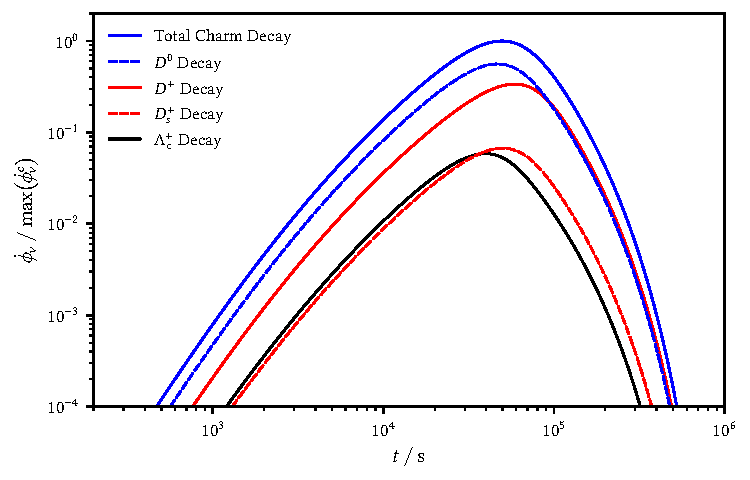
\includegraphics{../plots/build/magnetar_charm_decay_comparison_without.pdf}
	\caption[Magnetar $\nu \kern+0.5pt$ flux from $c$ decay excluding optical depth.]
			{Comparison of individual charmed hadron contributions to the total charm neutrino flux at
			 $E_\nu = \qty{e9}{\giga\electronvolt}$ from a newborn magnetar, excluding optical depth.}
	\label{fig:magnetar-charm-comparison-without}
\end{figure}


\begin{figure}[H]
	\centering
	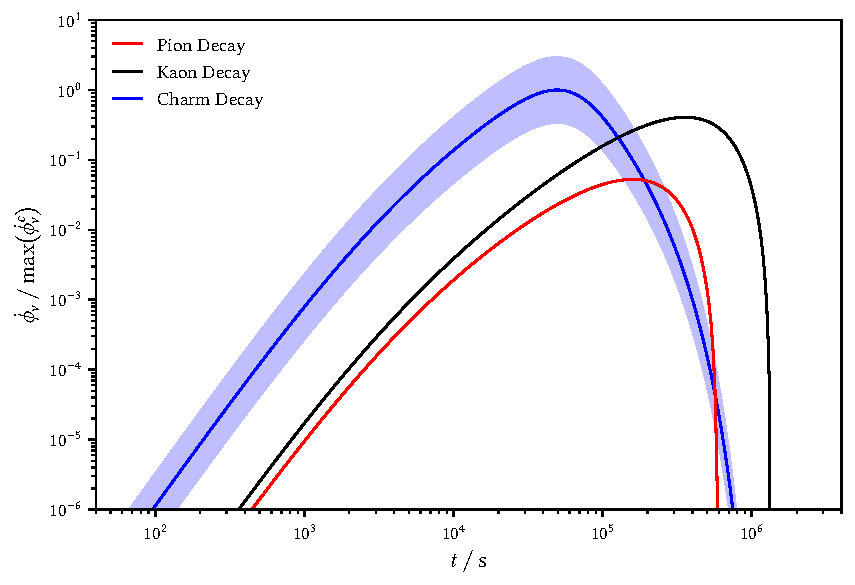
\includegraphics{../plots/build/magnetar_neutrino_spectrum_without.pdf}
	\caption[Magnetar $\nu \kern+0.5pt$ flux compared to $c$ decay without optical depth.]
			{}
	\label{fig:magnetar-flux-without}
\end{figure}

\begin{figure}[H]
	\centering
	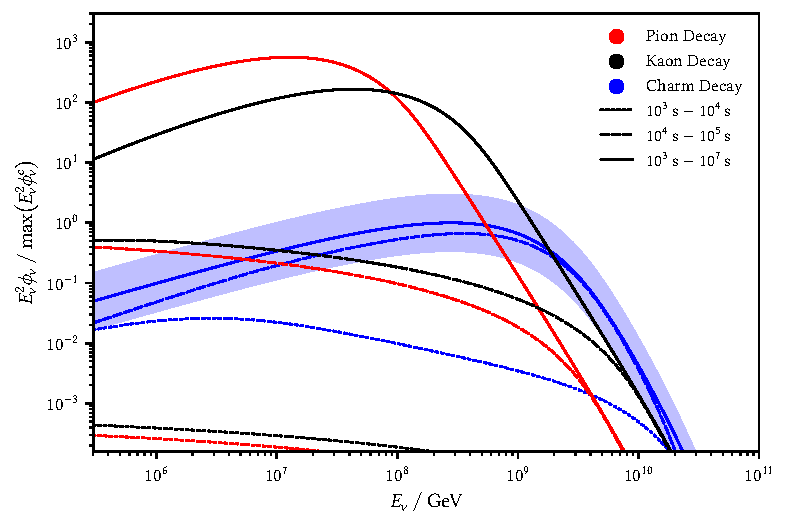
\includegraphics{../plots/build/magnetar_integrated_neutrino_spectrum_without.pdf}
	\caption[]{}
	\label{fig:magnetar-fluence-without}
\end{figure}


better agreement, shape, peaks with lifetime, 

\begin{figure}[H]
	\centering
	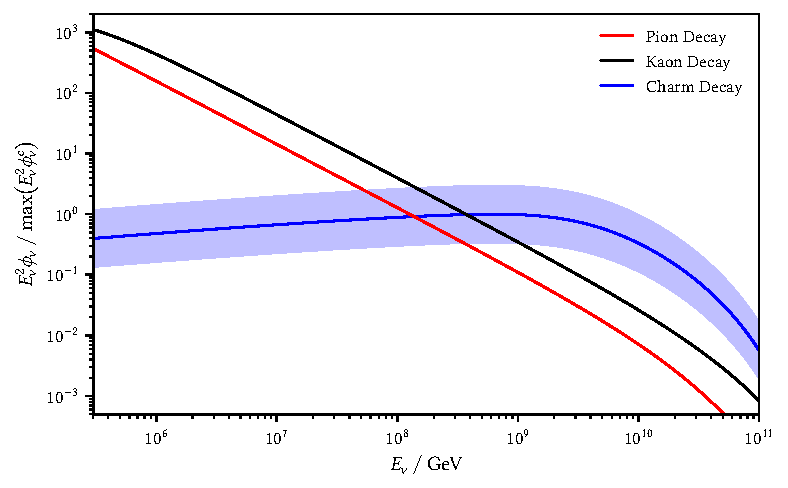
\includegraphics{../plots/build/nucleus_neutrino_spectrum.pdf}
	\caption[AGN accretion disk $\nu \kern+0.5pt$ fluence compared to $c$ decay.]
			{}
	\label{fig:nucleus-fluence}
\end{figure}

\begin{figure}[H]
	\centering
	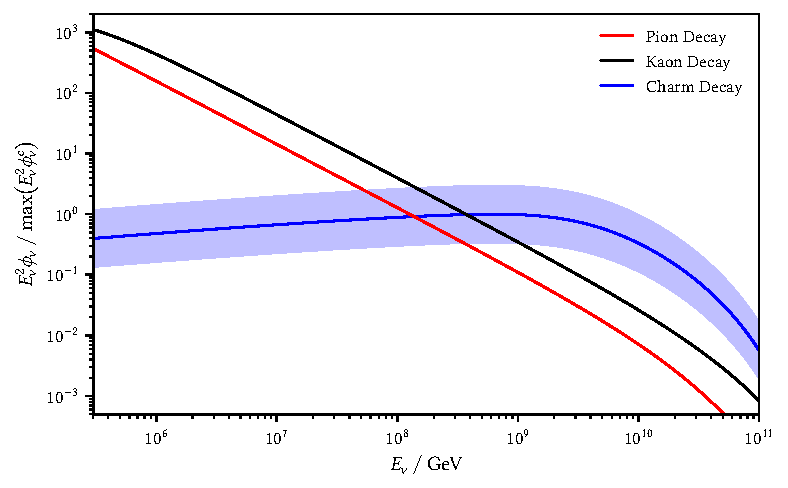
\includegraphics{../plots/build/nucleus_neutrino_spectrum.pdf}
	\caption[AGN accretion disk $\nu \kern+0.5pt$ fluence compared to $c$ decay.]
			{Expected neutrino fluence normalized to the maximum charmed hadron contribution from an AGN accretion disk.
			 Differences between the shapes of pion and kaon components compared to charm decays result from the chosen
			 view, as the flat increase observed for charmed hadrons occurs at lower energies in the case of pions and kaons
			 due to their much longer lifetimes. These decay times are listed in Sections \ref{sub:scattering} and \ref{sub:charm}
			 with Figure \ref{fig:nucleus-charm-comparison} giving the reasoning for effects of cooling. Charmed hadrons dominate
			 the fluence from $E_\nu = \kern-0.5pt \qty{e9}{\giga\electronvolt}$ and above, lining up with prior expectations. This
			 threshold is sensitive to varying densities, with lower values producing a shift towards higher energies. A hard cutoff
			 is enforced by $E_p = \kern-0.5pt \qty{e12}{\giga\electronvolt}$ as the maximum proton energy. The same shaded uncertainty
			 band as in Figure \ref{fig:magnetar-flux-with} for charm decays as well as the scaling by $E_\nu^2$ from
			 Figure \ref{fig:magnetar-fluence-with} are adopted.}
	\label{fig:nucleus-fluence}
\end{figure}

